\chapter{Continuous Probability Distributions}

When we talked about the probability distribution of the sum of two dice,  we assigned a probability to each of the 11 possibilities:

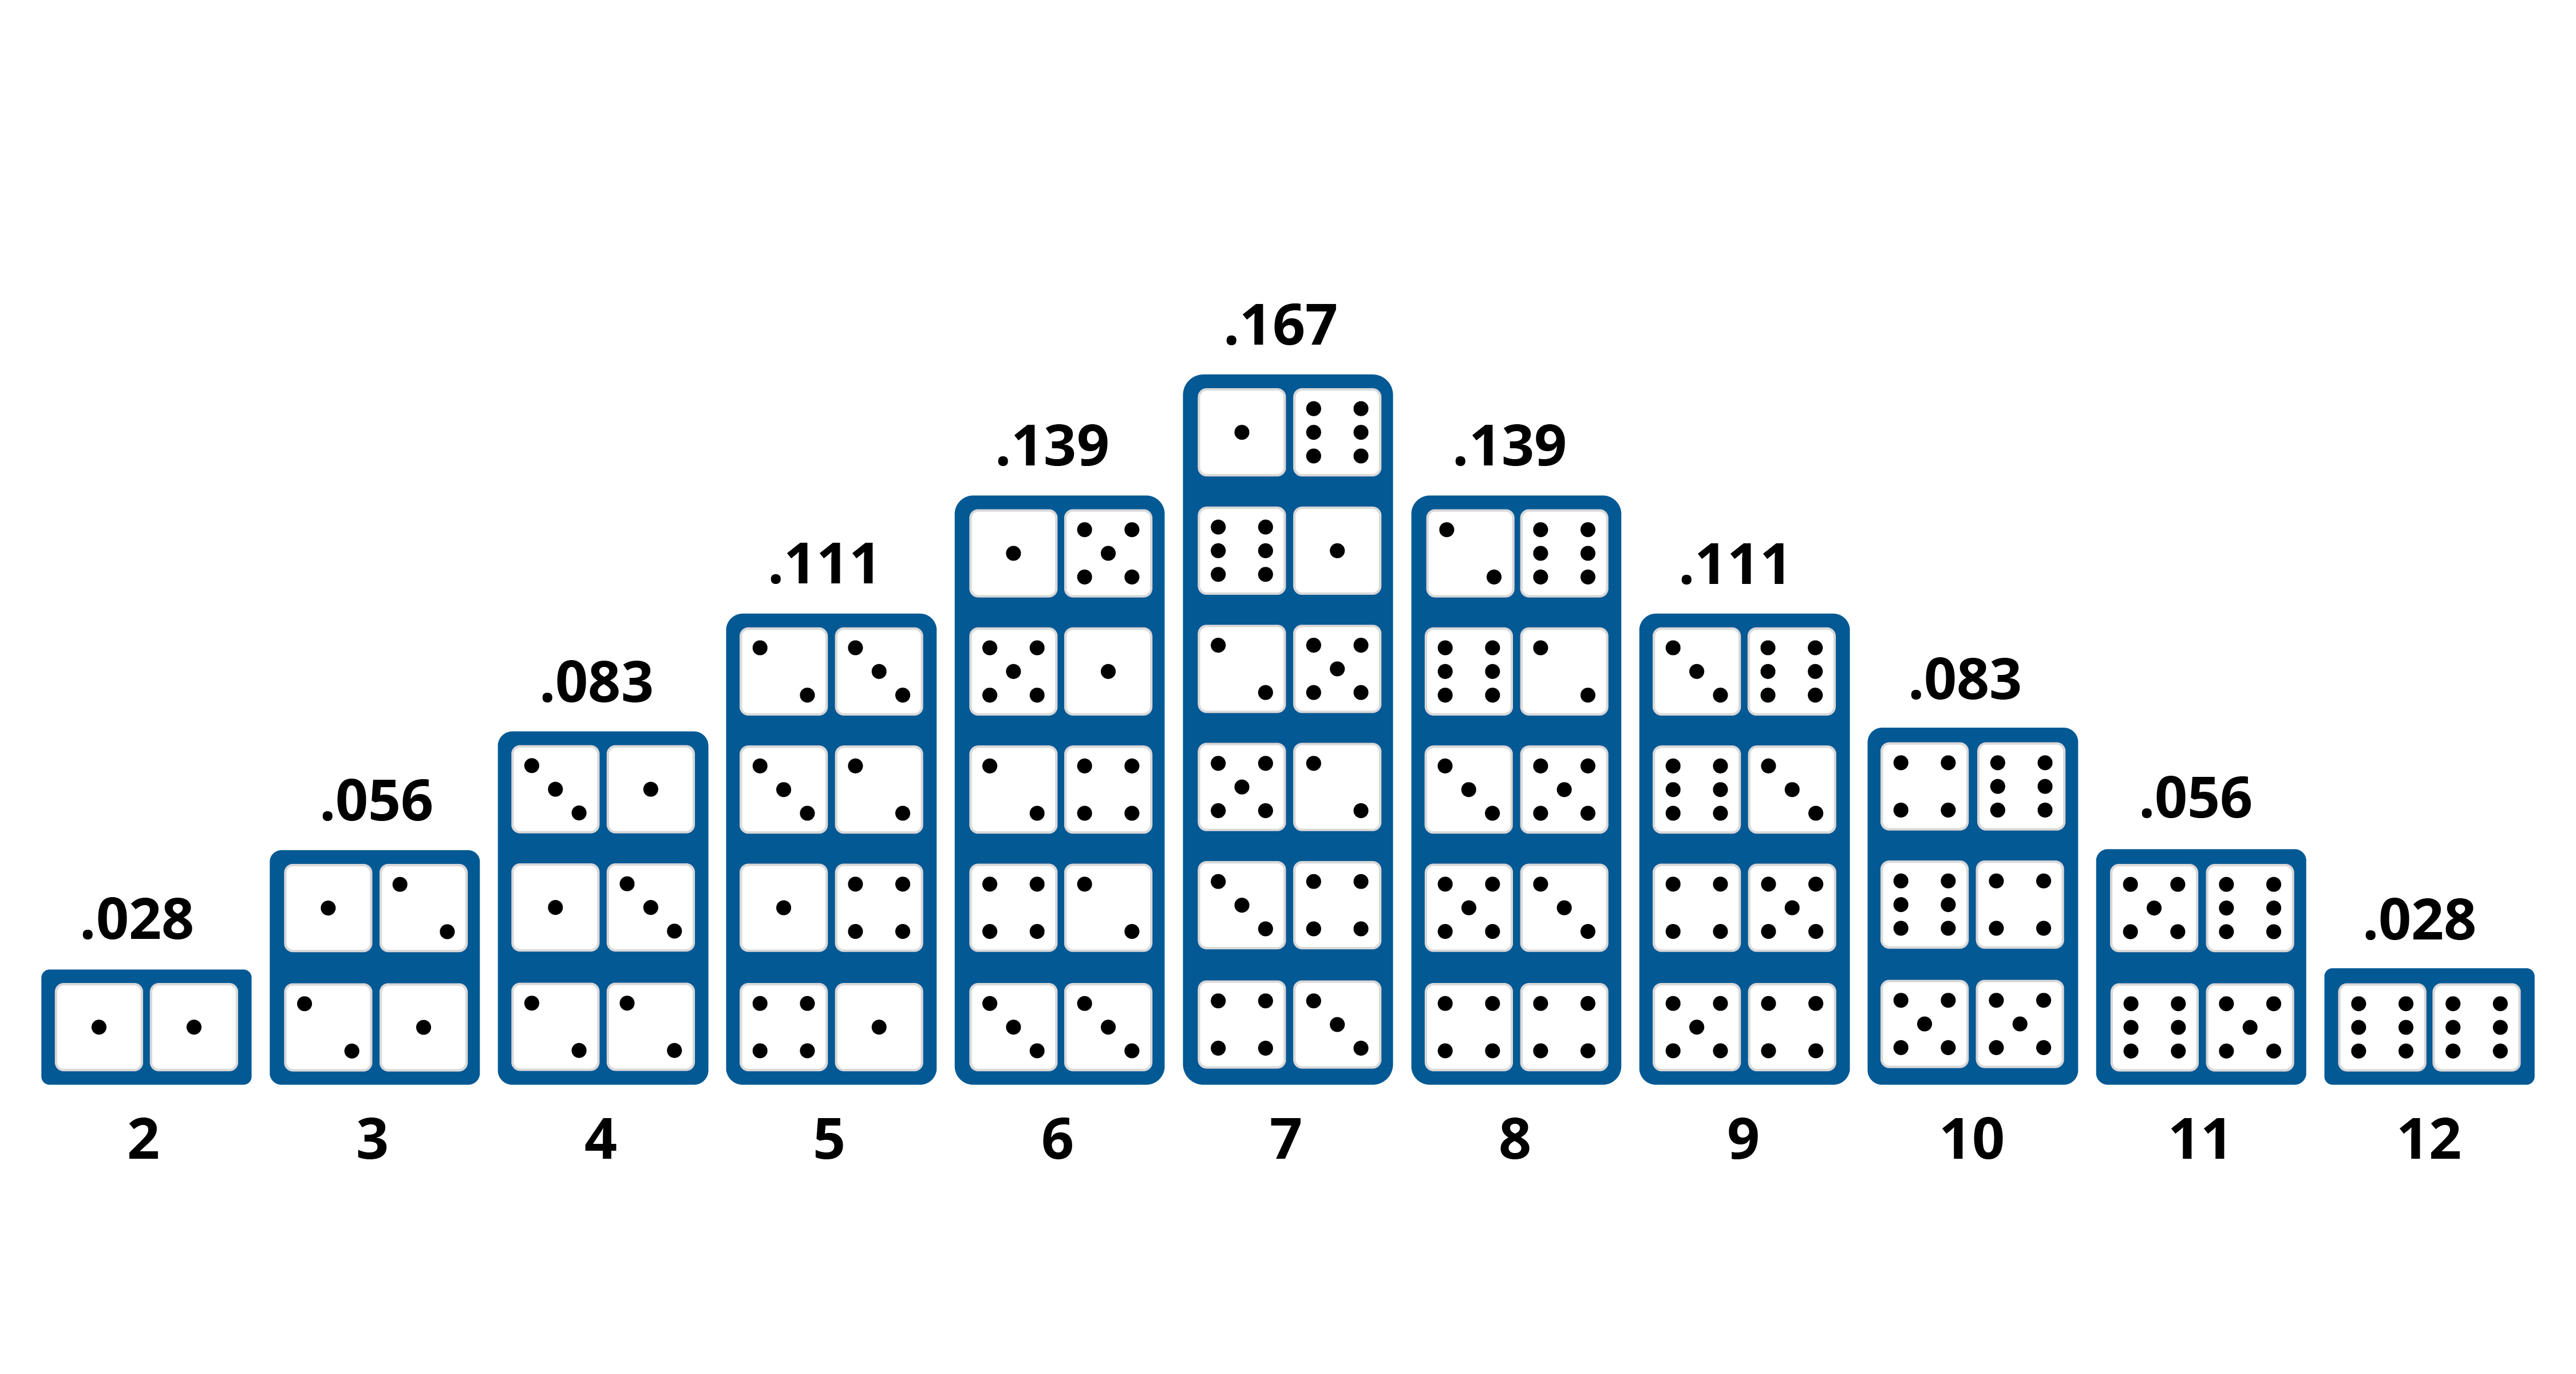
\includegraphics[width=0.7\textwidth]{dice_histogram.png}

The probabilities all added up to be 1.0.  That is a way of saying "100\% of the times you throw the dice,  the sum will be an integer between 2 and 12."

Now we need to talk about probabilities of properties that are continuous,  not discrete.   For example, we might want to ask the question "If I randomly pick a cow from all the cows in the 
world, what is the probability that it will weigh less than 597.34 kg?"  What does a probability distribution for a continuous variable look like?

\section{Cumulative Distribution Function}

Imagine that you live in ancient times.  You buy, sell, and ship cows.   A lot of people come into your office and brag about their cows: "Bessie is heavier than 99\% of the cows in 
world!"  So you need to develop some statistics on cow weights.

You have ten cows.  You weight them:

\begin{tabular}{c|r}
Cow & Mass in kg \\
\hline
Cow 1 & 580.22 \\
Cow 2 & 540.07 \\
Cow 3 & 538.20 \\
Cow 4 & 512.39 \\
Cow 5 & 589.75 \\
Cow 6 & 456.91 \\
Cow 7 & 583.09 \\
Cow 8 & 493.56 \\
Cow 9 & 489.97 \\
Cow 10 & 704.15 \\
\end{tabular}

If someone comes into your shop and says "My Bessie is an astonishing 530 kg!" it would be cool to have a list on the wall that would let you yell back "Half my cows are heavier than that, Silly!"  So you sort the cows by weight.  For each weight,  you say how many of your cows are lighter than that:

\begin{tabular}{c|r}
Proportion of cows lighter & Mass in kg \\
\hline
0.00 & 456.91 \\
0.10 & 489.97 \\
0.20 & 493.56 \\
0.30 & 512.39 \\
0.40 & 538.20 \\
0.50 & 540.07 \\
0.60 & 580.22 \\
0.70 & 583.09 \\
0.80 & 589.75 \\
0.90 & 704.15 \\
\end{tabular}

In fact, for easy reference,  you make a plot:

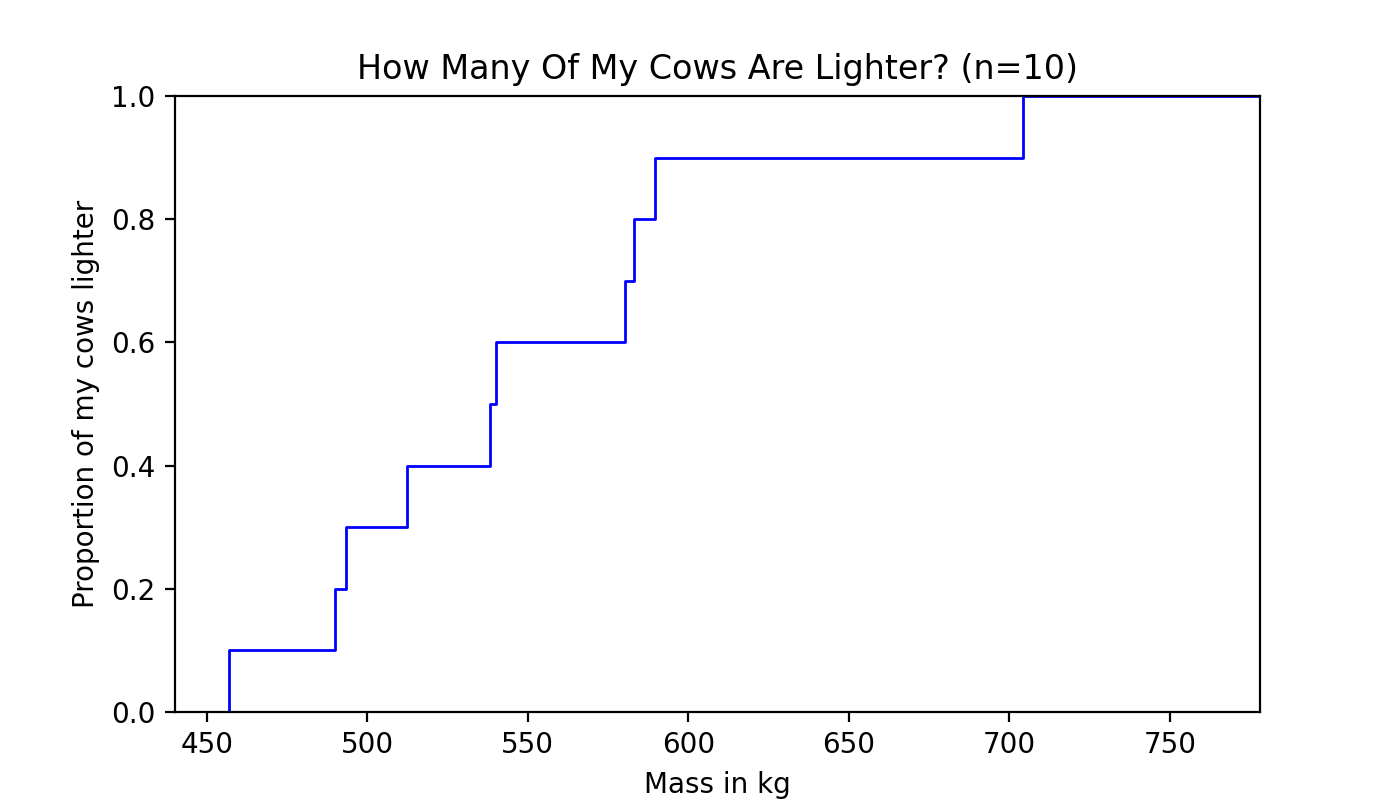
\includegraphics[width=0.7\textwidth]{cow_sample_cdf.png}

Now for any weight you can quickly look up what proportion of your cows are lighter.  (And, if you subtract that from 1,  what proportion of your cows are heavier.)

See how jagged that graph is?  That is because you only have the data for 10 cows.   However, as the years pass and you weight thousands of cows,  the plot will become smoother.   Because it
always accumulates more cows as you move from left to right,  this is known as a \newterm{cumulative distribution function} or CDF:

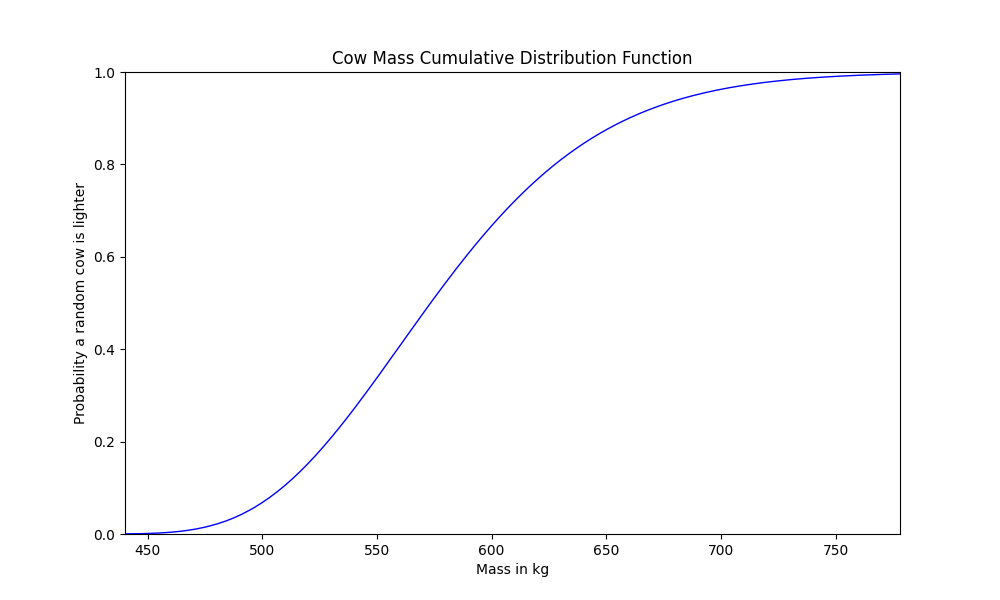
\includegraphics[width=0.7\textwidth]{cow_cdf.png}

A cumulative distribution function always starts at 0 and ends at 1.  On that journey, it never decreases.

Let's say you want to know what proportion of cows weigh between 620 kg and 635 kg.  Using the CDF, you could figure out that 77\% of all cows weigh less than 620 kg and 83\% of all cows 
weigh less than 635 kg.  Thus 6\% of all cows must weigh more than 620 kg and less than 635 kg.

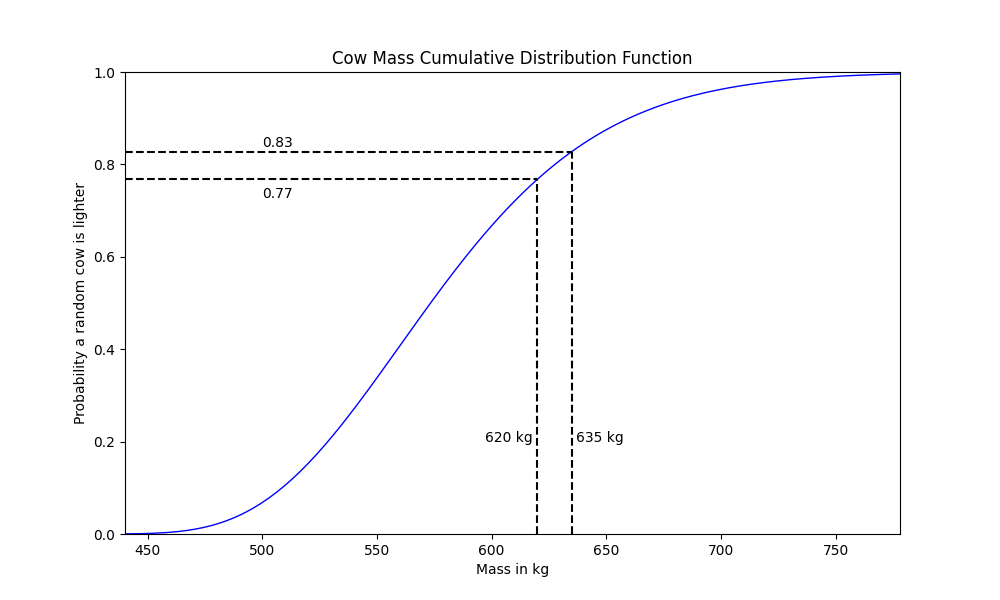
\includegraphics[width=0.7\textwidth]{cow_cdf_bounds.png}

\section{Probability Density Function}

The cumulative density function is handy,  but some of its information can be hard to see.  For example,  how would you answer the question "What is the most common weight of a cow?"  You would
squint at the CDF and try to determine where it was steepest.

To make these sorts of questions easier to answer,  we take the derivative of the CDF to get the \newterm{probability density function} (or PDF).  For the cows,  it would look like this:

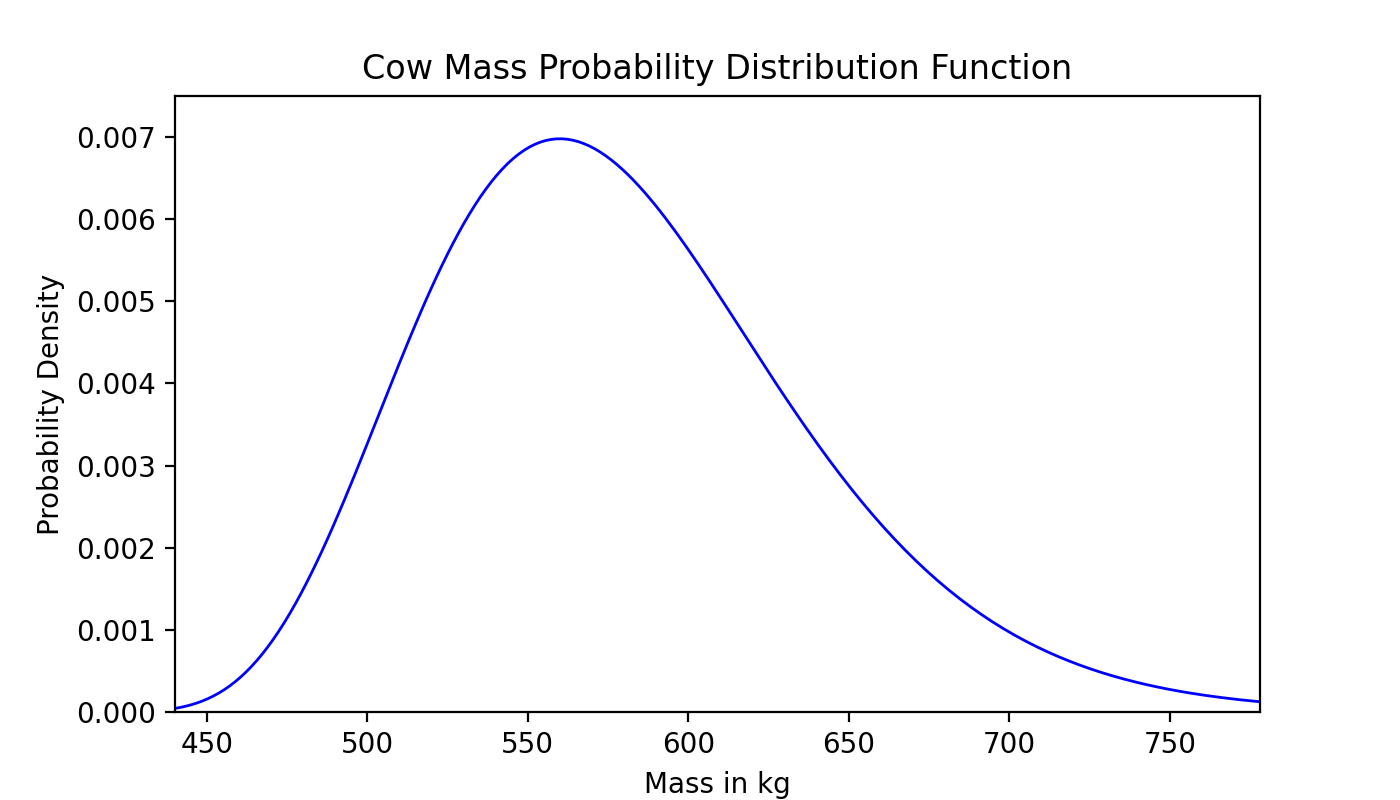
\includegraphics[width=0.7\textwidth]{cow_pdf.png}

Now you can easily see that the CDF was steepest at about 560 kg.  We call the highest point on the PDF the \newterm{most likely estimator}.  For example, you might say "560 kg is the most likely estimator of cow mass."  Sometimes we just say "the MLE".

Note that the MLE is often different from the mean or the median.  In this case, for example,  the distribution is skewed right -- there are more cows that are heavier than the 
MLE than there are cows that are lighter than the MLE.    The MLE would be less than the mean or the median.

Once again,  lets say you want to know what proportion of cows weight between 620 kg and 635 kg.   This is more difficult with a PDF than it is with a CDF.  With a PDF,  you have to find
the area under the curve between $x=620$ and $x=635$.  

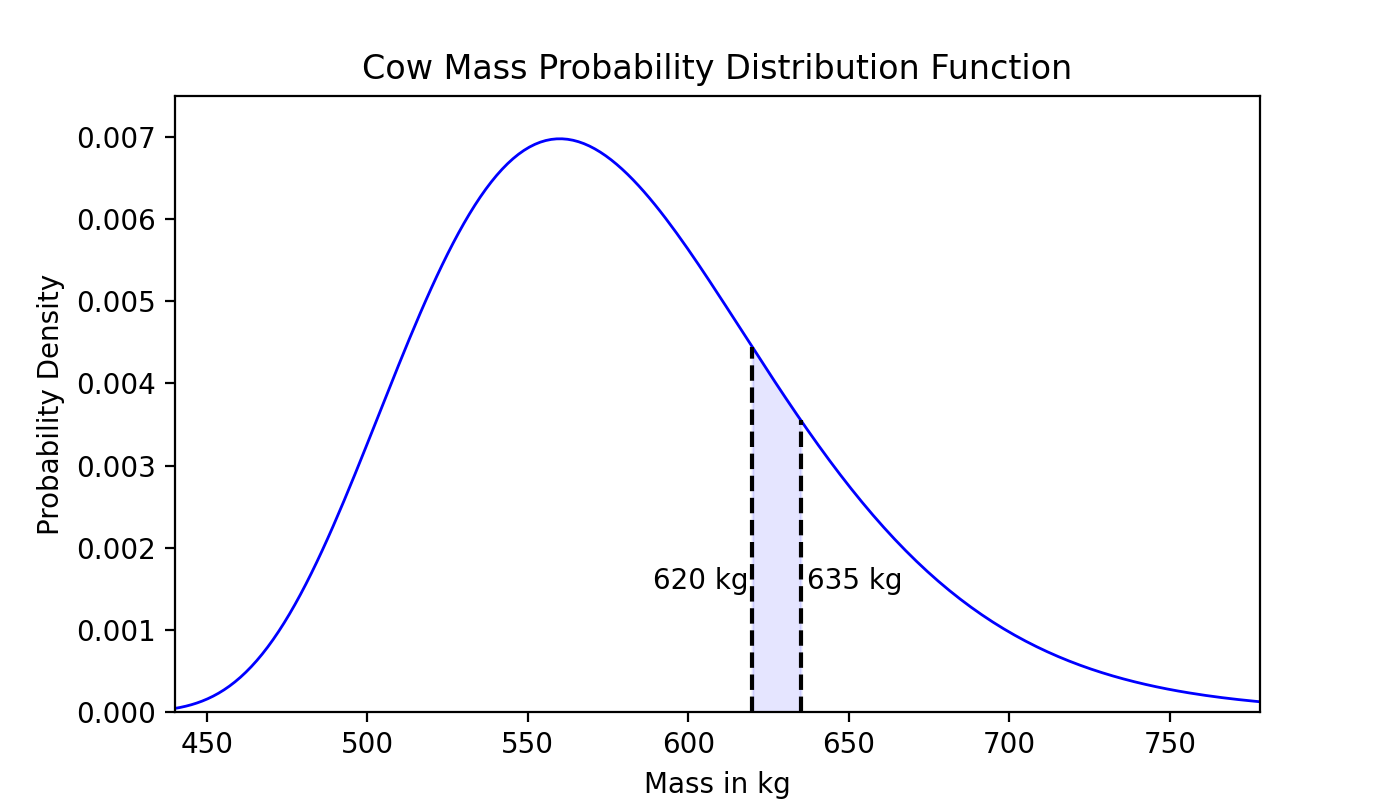
\includegraphics[width=0.7\textwidth]{cow_pdf_bounds.png}

This is why it is called a "probability density" -- to get a true probability you need to multiply the density by the width of the region.

What is the area under the entire curve?  If you integrated it, you would get the CDF.  The CDF goes from 0 to 1.0.   The area under a PDF is \emph{always} 1.0.

\section{The Continuous Uniform Distribution}

The most simple continuous distribution is the uniform distribution between two numbers $a$ and $b$.   The CDF is a straight line from zero at $a$ to 1 at $b$.  For example,
here is the CDF for the uniform distribution between 6 and 9.

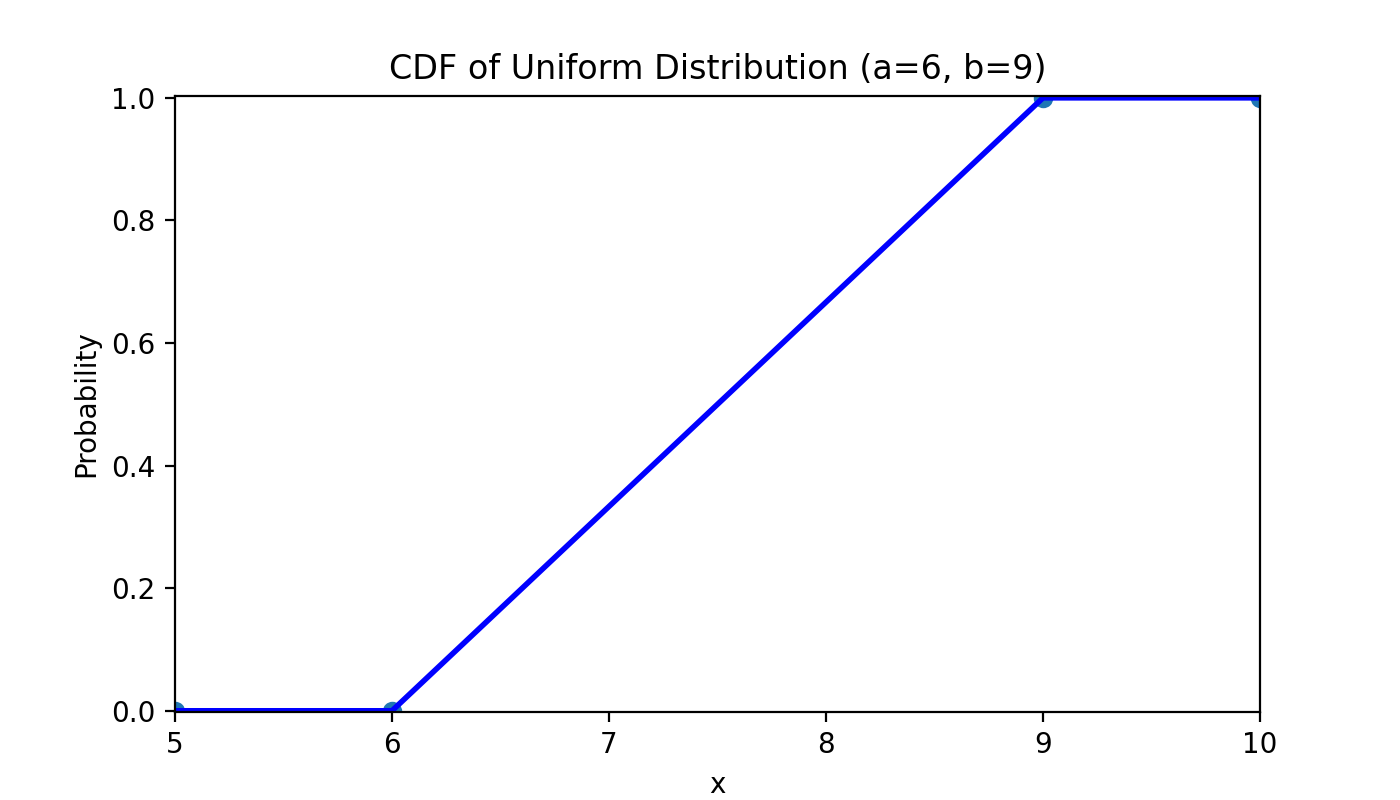
\includegraphics[width=0.7\textwidth]{unif_cdf.png}

That line goes from 0 to 1 over a distance of 3,   so its slope is $\frac{1}{3}$ between 6 and  9 and zero everywhere else.   Thus the PDF (its derivative),  looks like this:

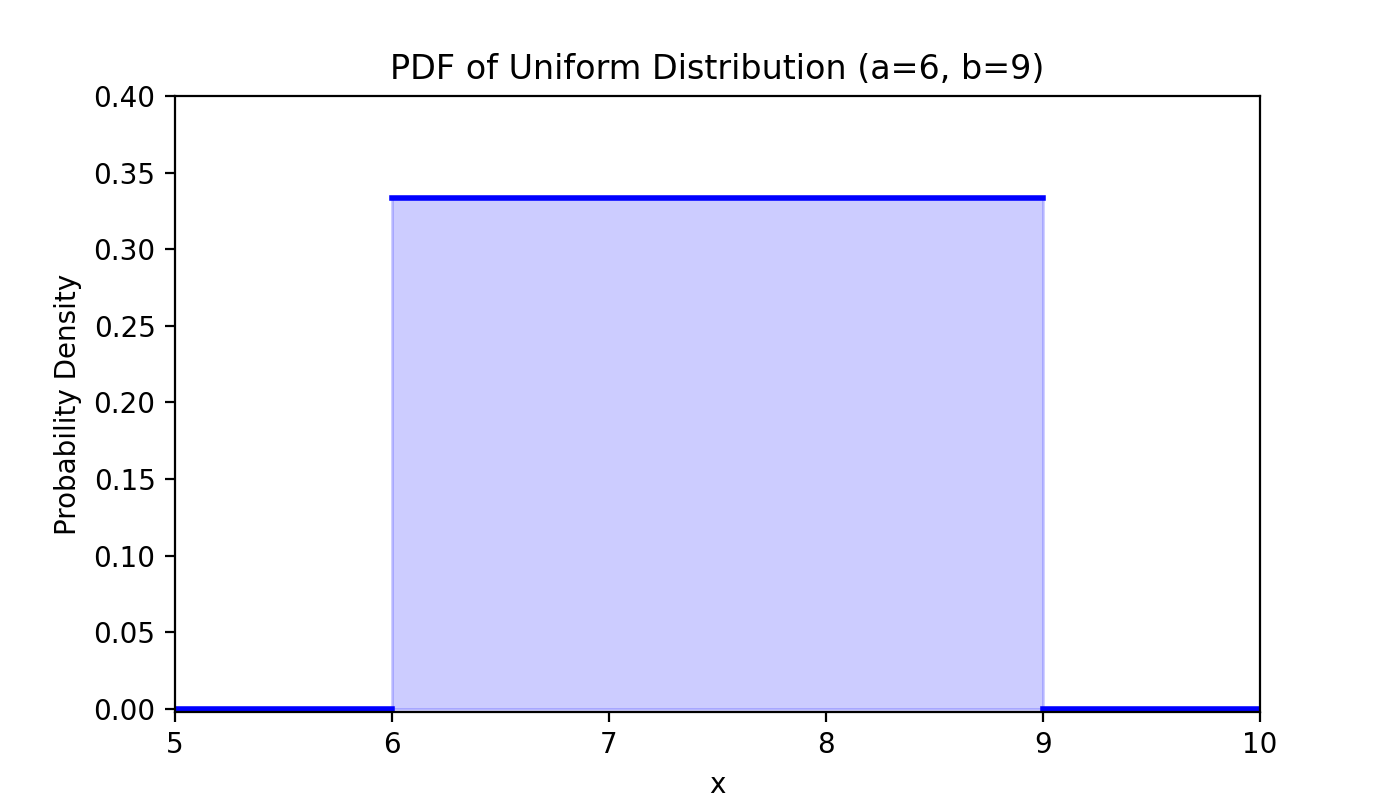
\includegraphics[width=0.7\textwidth]{unif_pdf.png}

So we can write the probability distribution of a continuous uniform distribution between $a$ and $b$ as:

  $p(x) = \begin{cases}
  \frac{1}{b-a} & \text{for } a \le x \le b, \\[8pt]
  0 & \text{for } x < a \ \text{ or } \ x > b.
  \end{cases}$

Notice that if $a$ and $b$ are less than 1 apart,  the value of $p(x)$ will be greater than 1.  This is a really important difference between a probability and a probability density: 
\begin{itemize}
\item A probability will always be in  the interval $[0, 1]$.  
\item A probability density will never be less than 0,  but can be much larger than 1.
\end{itemize}

That said,  the probability density will always integrate to 1.

Here is the PDF for a uniform distribution between 0.6 and 0.9:

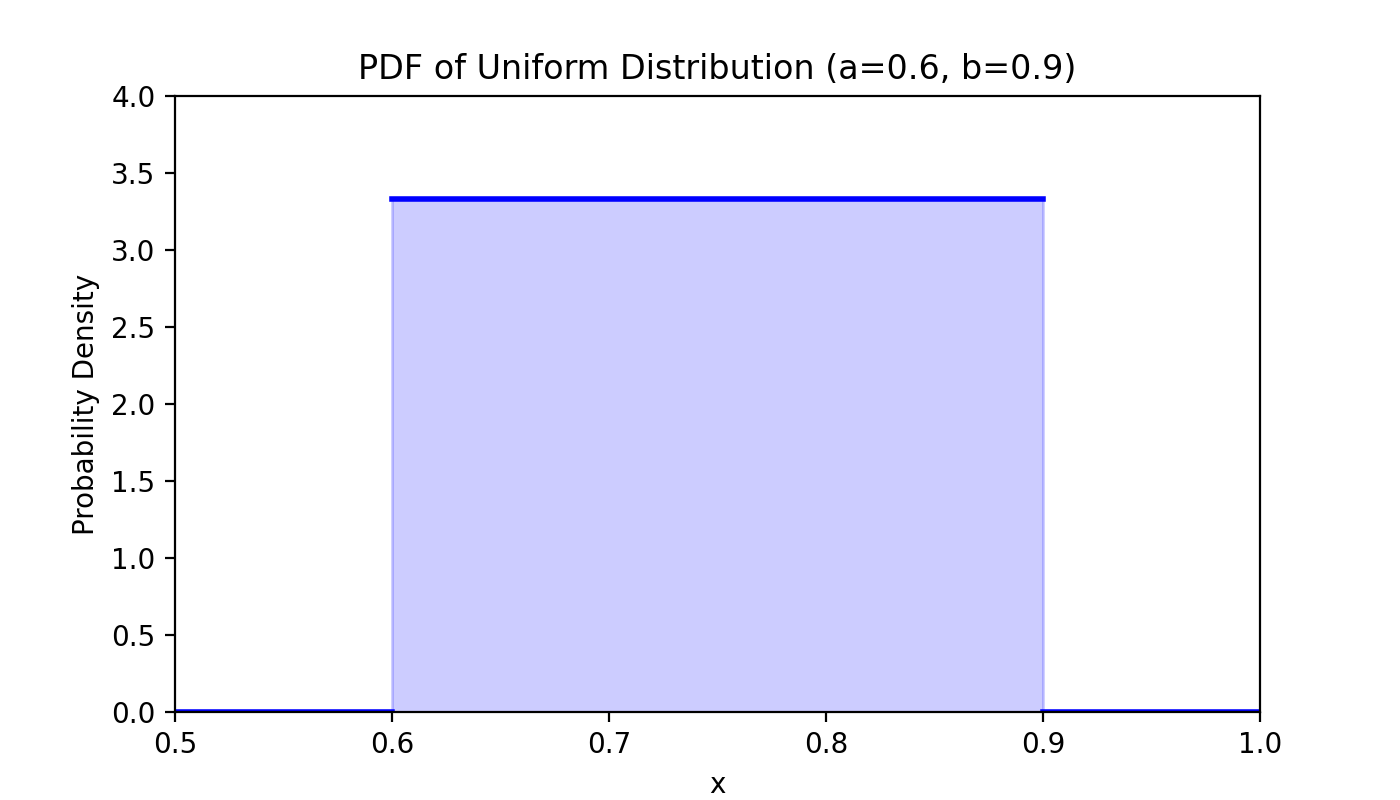
\includegraphics[width=0.7\textwidth]{unif_pdf2.png}

The mean and median of a uniform distribution between $a$ and $b$ is its midpoint:  $\frac{a+b}{2}$.

The variance ($\sigma^2$) is $\frac{(b -a)^2}{12}$.

\section{Continuous Distributions In Python}

The SciPy library has functions that let a programmer work with a large collection of different probability distributions.

For example,  if you wanted to work with a continuous uniform distribution between 6 and 9,  you would import the relevant
functions like this:

\begin{verbatim}
from scipy.stats import uniform
\end{verbatim}

Now if you wanted a numpy array containing a sample of 300 numbers generated randomly from that distribution:

\begin{verbatim}
samples = uniform.rvs(loc=6,  scale=3,  size=300)
\end{verbatim}

The \pyvar{loc} argument is $a$.  The \pyvar{scale} argument is $b - a$.

If you wanted to know the value of the probability density function at 8 and 10, you could use the \pyfunction{pdf} function:

\begin{verbatim}
x_values = np.array([8, 10])
p_values  = uniform.pdf(x_values,  loc=6,  scale=3)
\end{verbatim}

Now \pyvar{p\_values} contains 0.33333 and 0.0.

To get the value of the cumulative distribution function at those points,  you would use the \pyfunction{cdf} function:

\begin{verbatim}
cdf_values = uniform.cdf(x_values,  loc=6,  scale=3)
\end{verbatim}

Now \pyvar{cdf\_values} contains 0.666667 and 1.0.

The inverse of the CDF is very useful.   It answers questions like "How heavy does a cow have to be to be in top 1\%?"

\begin{verbatim}
bottom_top_percentiles = np.array([0.01,  0.99])
boundaries = uniform.ppf(bottom_top_percentiles,  loc=6,  scale=3)
\end{verbatim}

Now \pyvar{boundaries} contains 6.03 and 8.97.

The SciPy library supplies these functions (\pyfunction{rvs}, \pyfunction{pdf},  \pyfunction{cdf}, and \pyfunction{ppf}) for over a hundred 
common continuous probability distributions.   

The common "bell curve" shaped distribution is called a Gaussian  or Normal distribution.  It is described by its mean (the midpoint of the bell) and its standard deviation.   For the normal distribution,  the standard deviation is the distance you have to go from the mean to reach 68\% of the population. 
We will talk a lot more about the normal distribution in other chapters,  but lets take this opportunity to plot the CDF and PDF of a normal distribution with a mean of 32 and a standard deviation of 8.

Create a file called \filename{plot\_norm.py} and add the following lines:

\begin{verbatim}
import numpy as np
from scipy.stats import norm
import matplotlib.pyplot as plt

# Constants
MEAN = 32
STD = 8

# Plottin from the 0.5 percentile to the 99.5 percentile
x_min = norm.ppf(0.005, loc=MEAN, scale=STD)
x_max = norm.ppf(0.995, loc=MEAN, scale=STD)

# Make 200 points between x_min and x_max
x_values = np.linspace(x_min, x_max, 200)

# Get CDF for each x value
cdf_values = norm.cdf(x_values, loc=MEAN, scale=STD)

# Get PDF for each x value
pdf_values = norm.pdf(x_values, loc=MEAN, scale=STD)

# What is the highest density?
max_density = norm.pdf(MEAN, loc=MEAN, scale=STD)

# Make a figure with two axes
fig, axs = plt.subplots(nrows=2, sharex=True, figsize=(8, 8), dpi=200)
axs[0].set_xlim(left=x_min, right=x_max)

# Draw the CDF on the first axis
axs[0].set_title("CDF of Normal Distribution (mean=32, std=8)")
axs[0].set_ylim(bottom=0.0, top=1.0)
axs[0].plot(x_values, cdf_values)

# Draw the PDF on the second axix
axs[1].set_title("PDF")
axs[1].set_ylim(bottom=0.0, top=max_density * 1.1)
axs[1].plot(x_values, pdf_values)

# Add lines for mean,  mean-std, and mean+std
axs[1].vlines(MEAN - STD, 0, max_density, "r", linestyle="dashed")
axs[1].vlines(MEAN + STD, 0, max_density, "r", linestyle="dashed")

# Save out the figure
fig.savefig("norm_32_8.png")
\end{verbatim}

The resulting plot should look like this:

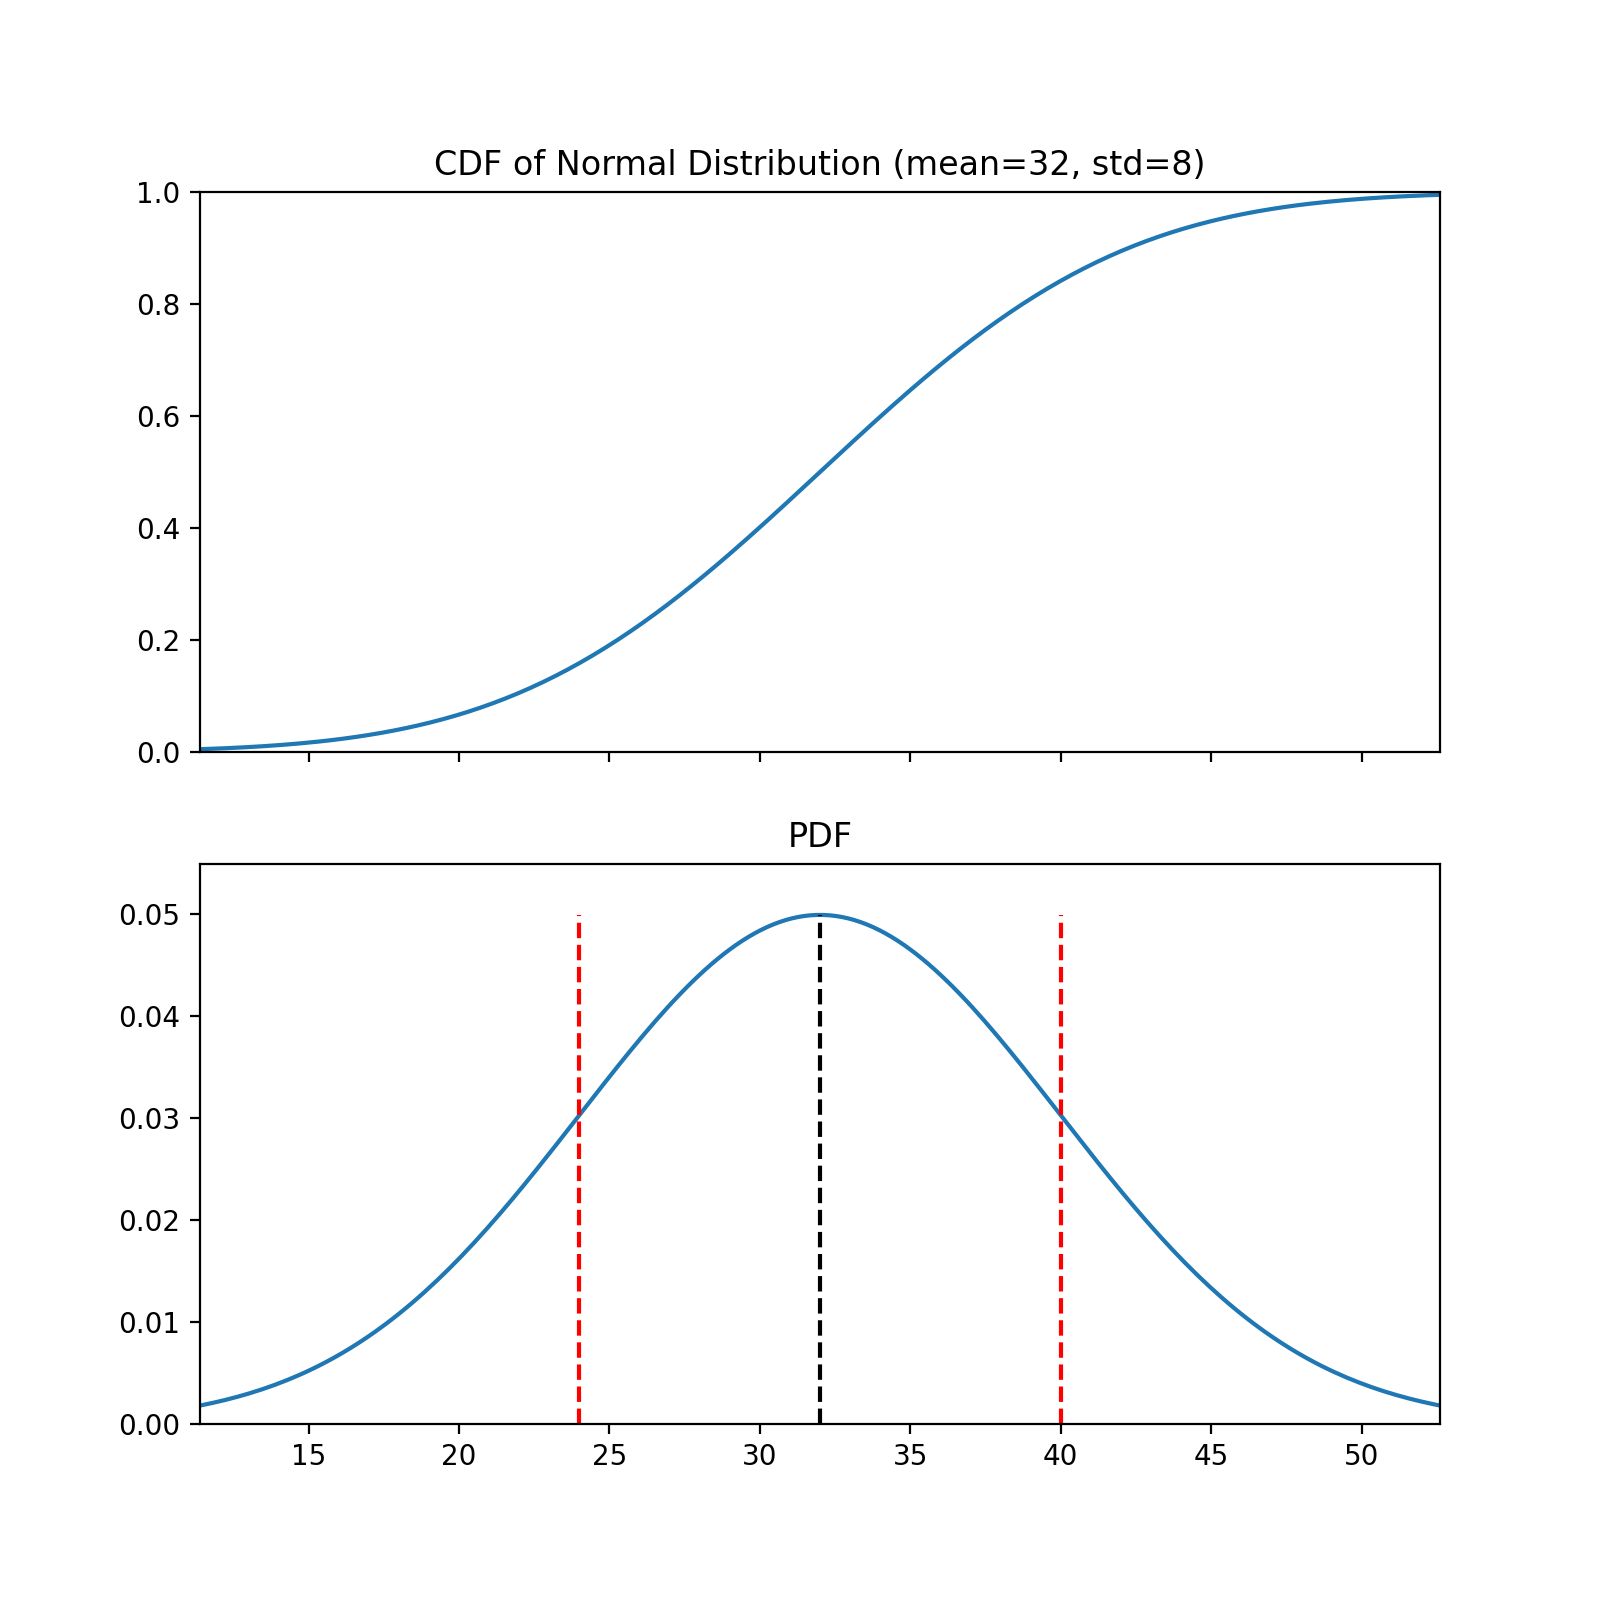
\includegraphics[width=0.7\textwidth]{norm_32_8.png}

What do those vertical lines mean?  An ornithologist might tell you "The wingspan of adult robins are normally distributed with a mean of 32 cm and a
 standard deviation of 8 cm."  Then 68\% of the population of adult robins would have wingspans between the two red lines.